%\chapter{Život během pandemie: Proměny chování a kontaktů a jakou roli hrají v epidemii}\label{Zmeny_chovani}
\chapter[Život během pandemie: Chování a kontakty]{Život během pandemie: Chování, kontakty a jejich proměny}\label{Zmeny_chovani}

\textit{Daniel Prokop, Michaela Kudrnáčová, Tomáš Hovorka, Eliška Dvořáková}
\vspace{15mm}

\section*{Epidemie jako sociální problém}

Epidemie koronaviru je nejen medicínský, ale i sociální problém. Výzkum \uv{Život během pandemie} ukazuje, že vedla k destabilizaci práce a dočasné ztrátě příjmů zejména u~lidí s méně stabilní pracovní pozicí v oblasti služeb a měla dopady na duševní zdraví obyvatel.\footnote{U těchto zjištění i v další části kapitoly odkazujeme k výzkumu, jehož data jsou veřejně dostupná na webu \url{www.zivotbehempandemie.cz}}  Podle rodičů a učitelů se distanční vzdělávání podepsalo i nižší motivací dětí.\footnote{PAQ Research a Kalibro: Zkušenosti českých učitelů s~distanční výukou. On-line: \url{https://www.paqresearch.cz/post/zkusenosti-ceskych-ucitelu-s-distancni-vyukou}} Ale nejde pouze o~dopady. I~pro pochopení šíření epidemie je nutné znát sociologická data. Jak se mění aktivity lidí? Jak se scházejí? Využívají zaměstnavatelé home office? Jak se s ohledem na tyto věci mění počty kontaktů, které úzce souvisejí s vývojem reprodukčního čísla (viz Duševní zdraví na straně \pageref{Dusevni_zdravi})? Jaká je struktura těchto kontaktů (např. z~hlediska setkávání generací) a kde se odehrávají?

To vše je nutné znát pro efektivní designování protiepidemických opatření. V pozd\-ních fázích epidemie bylo naopak klíčovou znalostí, jak se vyvíjí ochota k vakcinaci a později také, kolik lidí z různých skupin získalo alespoň částečnou imunitu očkováním či proděláním nemoci a jak se díky tomu mění počet mezilidských kontaktů, při nichž ani jeden z aktérů není před onemocněním covid-19 částečně chráněn.

Kvůli těmto i dalším otázkám sociologové výzkumné společnosti PAQ Research v březnu 2020 založili longitudinální výzkum \uv{Život během pandemie}, ve kterém na panelu 2100 až 2500 respondentů sledují vývoj chování a dopadů epidemie.

V následující kapitole shrneme jeho základní zjištění. Nejprve popíšeme základní metodiku výzkumu, následně se budeme věnovat dopadům na domácnost a proměnám chování, vývoji kontaktů a modelování, kde se tyto kontakty odehrávají a jak do jejich významu zasahuje očkování.

\section*{\uv{Život během pandemie}: Základní informace}

Výzkum je unikátní především právě svou longitudinalitou. Počínaje březnem roku 2020 proběhlo první šetření a od té doby se v horizontu 2–3 týdnů pravidelně opakuje. Do konce května 2021 máme k dispozici již data z 28. vlny. Dotazován je stále stejný reprezentativní vzorek čítající v jednotlivých vlnách 2100 až 2500 respondentů. Díky této dlouhodobé metodice je možné zkoumat změny chování stejné skupiny domácností (vývoj není dán změnami samplingu), ale hlavně odpovídat na otázky typu: O~kolik se u~českých pracujících změní počet kontaktů, když přejdou na home office? Jak se do postojů a chování promítá to, když člověk covid-19 prodělá či mu zemře někdo blízký? Jaké typy aktivit souvisejí s vyšší pravděpodobností infekce?

Sběr dat výzkumu \uv{Život během pandemie} má „deníkový“ charakter – respondenti v něm reportují vždy o~svých aktivitách, pracovním životě, chování v uplynulém týdnu (či v některých případech dvou týdnech). Poskytují také informace o~tom, zda v tomto období prošli očkováním či testováním, a reportují svoje aktuální postoje či symptomy nemoci. Šetření kvůli tomu a dalším důvodům probíhá on-line.\footnote{Dotazování však také musí probíhat rychle – většina respondentů tento „deníkový“ záznam provede hned při startu vlny v pondělí, off-line šetření by takovou metodu neumožňovala. Doba epidemie neumožňovala face-to-face šetření. On-line šetření také jako jediné umožňuje uchovat vysokou retenci – tedy zhruba stejný vzorek respondentů po dobu více než 20 vln výzkumu. On-line dotazování také redukuje zkreslení odpovědí sociální desirabilitou (neochota přiznat některé postoje a porušování pravidel v přítomnosti tazatele). K~zajištění kvality odpovědí jsou dotazníkem prolnuty kontrolní otázky, vyhodnocující nepozorné vyplňování, a taktéž celkový čas strávený vyplňováním dotazníku prochází kontrolou. } Výzkum je kvótně reprezentativní pro populaci ČR z hlediska všech sociodemografických proměnných, kraje, velikosti obce a pracovního statusu.\footnote{Pracovní status – zaměstnanec, OSVČ, důchodce a ostatní.} Účastnit se ho však mohou jen lidé s~připojením k internetu – což do jisté míry omezuje výpovědní hodnotu o~populaci nad 60 let. Negativní vliv tohoto vychýlení se snažíme redukovat mj. tím, že je vzorek dovážen na dospělou populaci i z hlediska kombinace věku a vzdělání. Mezi staršími respondenty jsou tedy nadreprezentováni ti vzdělanější, což je obvyklý důsledek on-line sběrů dat.

Hlavní výstupy spolu s přehlednou vizualizací dat jsou dostupné na WWW stránkách \url{https://www.zivotbehempandemie.cz}. Na projektu pracují výzkumníci ze společnosti PAQ Research spolu s vědci z iniciativy IDEA AntiCovid a BISOP. Data jsou sbírána agenturou NMS na Českém národním panelu.

\section*{Ekonomické dopady na domácnosti}
\label{Ekonomicke_dopady}

Epidemie koronaviru přinesla vyšší dopady na pracovní život, než ukazují oficiální statistiky nezaměstnanosti. Během první vlny na jaře 2020 sice nestoupl počet zcela nezaměstnaných, ale řada pracujících se potýkala s~omezením práce. Část z~toho byly výpadky práce spojené s kompenzací (překážky práce s~částečnou náhradou mzdy, přechod na ošetřovné či nucená dovolená), zčásti šlo o~omezení bez finanční náhrady (zejména snížení úvazku, ztráta stabilní práce). V~jedné chvíli se tak počet lidí s~omezením v~práci zvýšil z~předkrizových 8 na 27\,\% v rámci skupiny 18 až 64 let. V~létě 2020 nastalo oživení, ale podzimní vlna opět přinesla zvýšený výskyt kompenzovaných omezení, který ustoupil až koncem dubna 2021. Dopad dalších vln byl ve srovnání s~první celkově slabší, ale zejména pracovníci z~obchodu a služeb a živnostníci byli dlouhodobě výrazně zasaženi. Epidemie se projevila také odchodem více lidí do ekonomické neaktivity (např. do důchodu). Během května roku 2021 bylo mezi lidmi od 18 do 64 let stále méně pracovně aktivních bez omezení práce (64\,\%), než tomu bylo před začátkem epidemie (69\,\%). Celkově ale pracovní trh nikdy nedostal tak výrazný zásah jako na jaře 2020 a programy Antivirus\footnote{Jde o~program ochrany zaměstnanosti, který vznikl za účelem ochrany pracovních míst ve firmách. Prostřednictvím Úřadu práce stát kompenzuje firmám vyplacené prostředky, aby lépe zvládly pandemickou situaci bez nutnosti propouštění zaměstnanců.} omezily nárůst nezaměstnanosti za cenu kompenzovaného omezení pracovní aktivity.

Některé skupiny obyvatel byly koronavirovou krizí zasaženy ve větší míře než jiné. Týká se to především respondentů pracujících v sektoru obchodu a služeb. V této skupině také došlo k nejvyššímu nárůstu nekompenzovaného omezení práce – tedy různých omezení úvazků a výpadku práce OSVČ. K nejvýraznějšímu omezení pracovního života došlo mezi lidmi, kteří pracují na dohodu nebo měli část úvazku vyplácen tzv. na ruku (týká se cca 7\,\% pracujících). V rámci této skupiny se podíl lidí, kteří přešli do nezaměstnanosti či měli nekompenzované omezení práce na začátku epidemie, zvýšil o~zhruba 18 procentních bodů a doposud se nedostal do původní pozice.

V důsledku uzavření ekonomiky a výrazného omezení příjmů se na jaře 2020 výrazně zvýšil podíl dospělých osob dočasně žijících pod hranicí chudoby (tedy pod hranicí 60\,\% ekvivalizovaného mediánového příjmu domácností). Během první vlny došlo k nárůstu
příjmové chudoby v české společnosti z 10\,\% na dvojnásobek. Od září 2020 do května 2021 žilo pod hranicí chudoby 10 až 12\,\% respondentů, podíl osob ohrožených příjmovou chudobou se tedy vrátil na přibližně stejné hodnoty jako před vypuknutím epidemie.

Opět se však výrazně liší dopady na různé skupiny obyvatel. Na důchodce epidemie, až na výjimky, výrazně ekonomicky nedopadla. Pro OSVČ byly typické velké výkyvy příjmů v čase, které reagovaly na uzavírky a vypisování kompenzačních bonusů. Zaměstnanci se v průběhu pandemie díky postupnému ukončení programů Antivirus a snížení zdanění práce dostali do mírně lepší příjmové situace než před pandemií. Dlouhodobějším a výraznějším dopadům musí čelit osoby vydělávající si na dohodu či dostávající část příjmu na ruku. V dubnu 2020 se u~nich výskyt pod hranicí chudoby zdvojnásobil. I~v květnu 2021 žilo téměř 20\,\% jejich domácností pod hranicí chudoby, kdežto před začátkem pandemie to bylo jen 13\,\%.


\begin{figure}[ht]
    \centering
    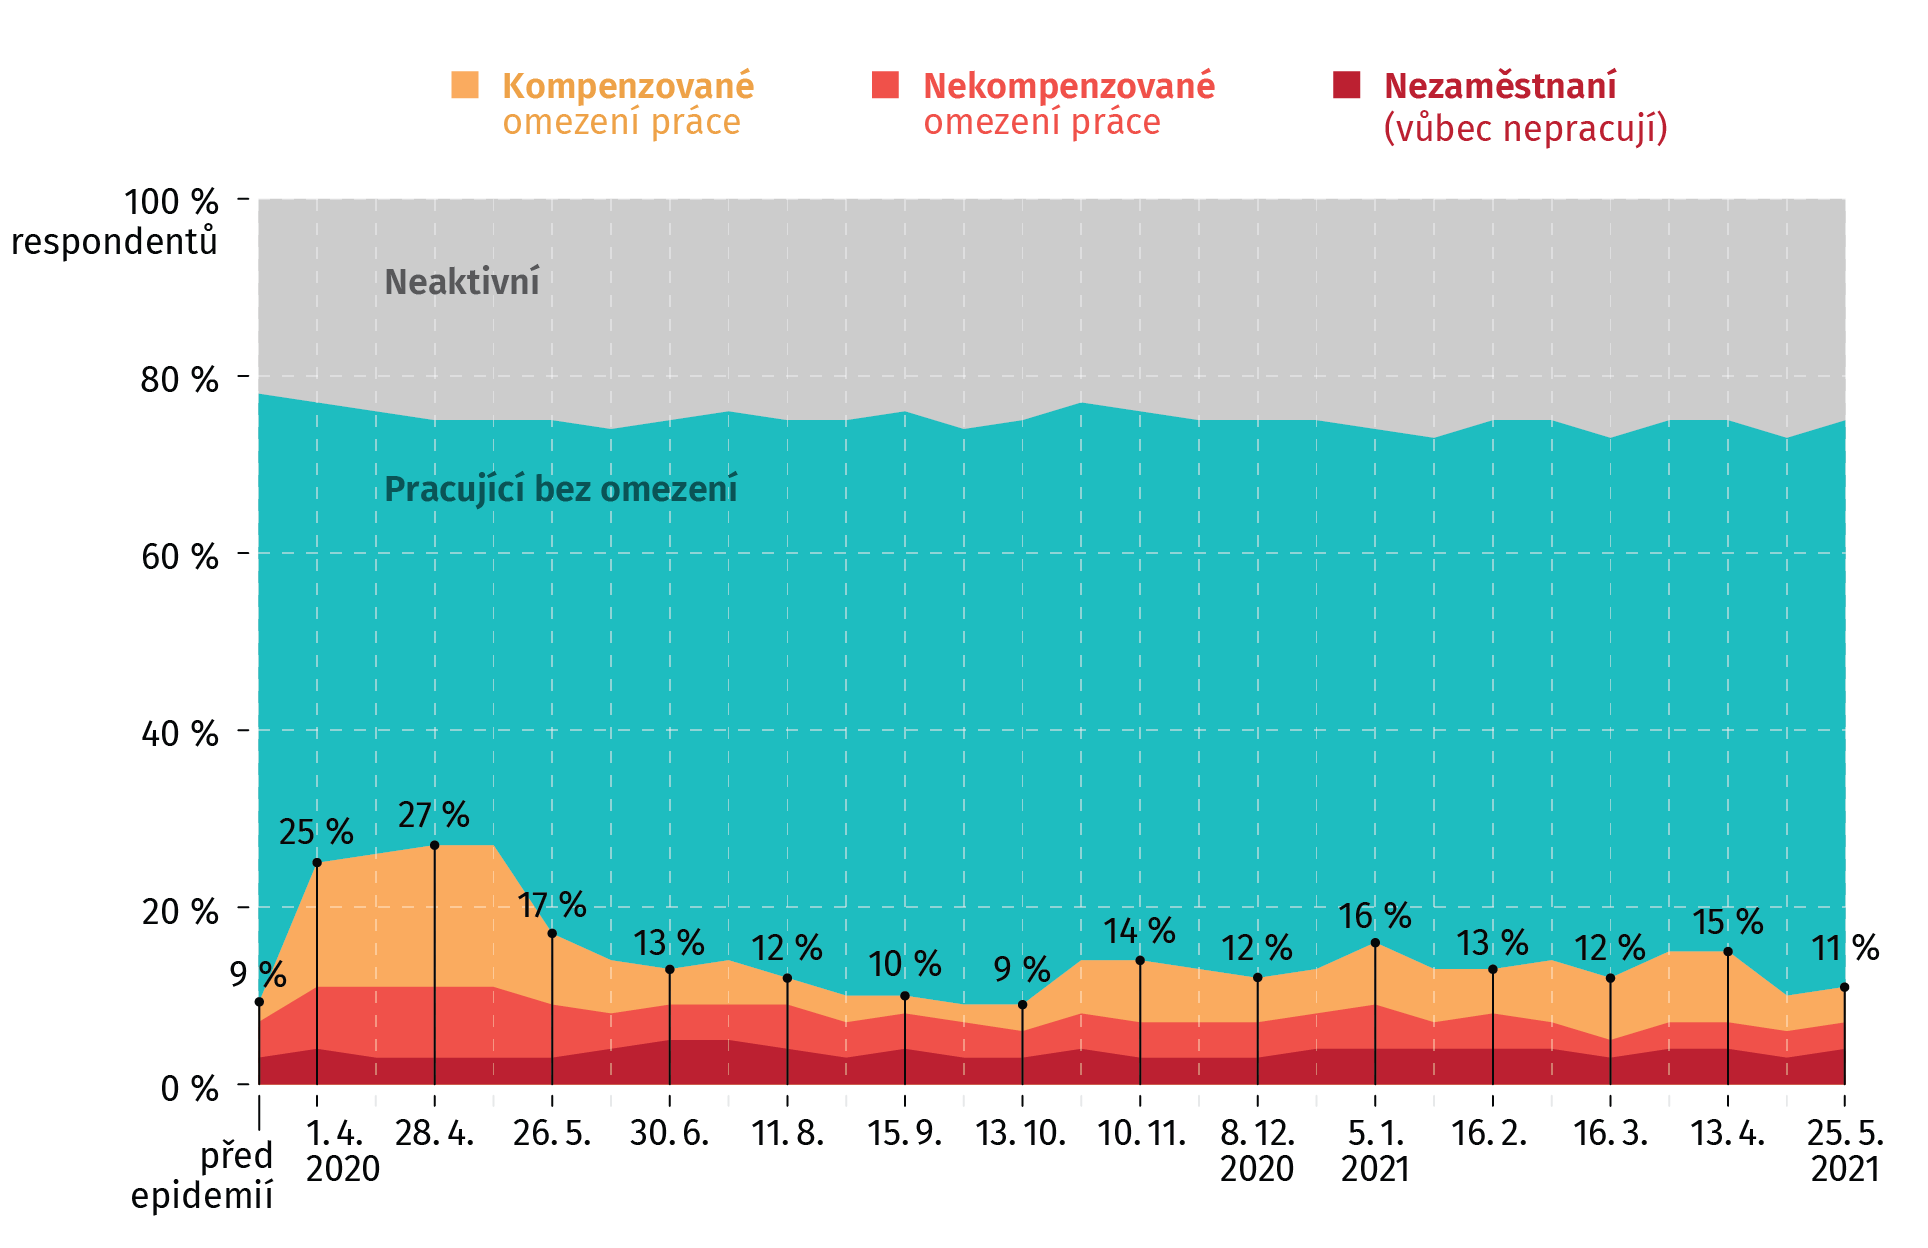
\includegraphics[width=0.9\textwidth]{./pic/zbp-graf1.png}
    \caption{Destabilizace práce během pandemie (respondenti 18--64 let).}
    \label{fig:zbp1}
\end{figure}

Kompenzované omezení práce: zaměstnanci nebo OSVČ dostávající částečnou náhradu mzdy (jsou na překážkách práce, v~karanténě apod.) jsou na ošetřovném nebo mají nucenou dovolenou. Nekompenzované omezení práce: zaměstnanci nebo OSVČ pracující omezený počet hodin (do 32 týdně), protože jim zaměstnavatel snížil úvazek či nemohou plně provozovat své podnikání, ztratili stabilní práci a nahrazují ji brigádami/sezonními pracemi nebo přišli o~příjmy na dohodu apod. Nezaměstnaní: nezaměstnaní, kteří v~posledních dvou týdnech nepracovali ani jednu hodinu. Pracující bez omezení: zaměstnanci nebo OSVČ, kterých se netýká žádné z~výše uvedených omezení práce. Neaktivní: studenti, důchodci, rodičovská.

\section*{Duševní zdraví}
\label{Dusevni_zdravi}

Nejistoty dané ekonomickou situací, zdravotními dopady, sociální izolací a obavami z budoucího vývoje mohou významně působit na psychiku člověka. Ve spolupráci s vědci z~IDEA Anti-Covid byly u~respondentů zjišťovány jejich pocity a obavy z probíhající epidemie a současně i jejich duševní zdraví. To je u~respondentů \uv{Života během pandemie} sledováno od začátku dubna 2020 baterií šesti klíčových otázek z široce používaných dotazníků PHQ8 a DAG7, které slouží jako základní sebediagnostický nástroj příznaků deprese a úzkosti. Respondent v nich odpovídá na otázky typu, jak často nemůže spát, zda ho nic nebaví a podobně. Výsledky této baterie nelze brát jako klinickou diagnózu depresí či úzkostí, ale jak ukazuje validační analýza IDEA, výsledky výrazně korelují s výsledky kompletních a detailnějších diagnostických nástrojů, které byly zařazeny do výzkumu jen v několika vlnách.\footnote{Viz
\url{https://idea.cerge-ei.cz/files/IDEA\_Dusevni\_zdravi\_covid-19\_cervenec2020\_22/IDEA\_Dusevni\_zdravi\_covid-19\_cervenec2020\_22.html\#p=1}}

Aby bylo možné vyhodnotit změny způsobené koronavirovou krizí, byli respondenti v prvních vlnách výzkumu jednorázově dotázáni na potíže – symptomy, které je sužovaly dva týdny před propuknutím krize. Příznaky alespoň středně těžké deprese či úzkosti v~době před epidemií podle této retrospektivní informace vykazovalo 6\,\% českých dospělých, což odpovídá i jiným odhadům. Na přelomu března a dubna uvedlo již 19\,\% respondentů příznaky alespoň středně těžké deprese či úzkosti, došlo tedy k~nárůstu způsobenému propuknutím epidemie na trojnásobek. Poté začal podíl dospělých osob s příznaky alespoň středně těžké deprese či úzkosti klesat až na prázdninových 8\,\%. Na podzim tento podíl tvořil 11\,\% respondentů a v únoru až dubnu 12 až 13\,\% dospělých. Od počátku května se výskyt příznaků ustálil na 10–11\,\% respondentů.

Koronavirová krize se velice podepsala na duševním zdraví žen s dětmi v~do\-mác\-nos\-ti. U~mužů se symptomy depresí a úzkostí v době epidemie měnily méně a přítomnost dětí v domácnosti u~nich nehraje zásadní roli. U~žen s dětmi vzrostlo v první vlně epidemie na jaře 2020 zastoupení těch, které vykazovaly příznaky středně těžké deprese či úzkosti, až na 37\,\%. V každé další vlně pak vidíme nárůst na 20 až 25\,\%. V rámci žen hraje velkou roli, zda mají děti v domácnosti (o~10--15 procentních bodů vyšší pravděpodobnost symptomů depresí a úzkostí). S jejich duševním zdravím jistě souvisí uzavření základních a mateřských škol, které přineslo větší zátěž spojenou s distanční výukou, ale i pokles příjmů v rámci tzv. ošetřovného.

Symptomy depresí či úzkostí často reportovali lidé z~nejmladší věkové kategorie do 24 let. Během dubna byly zaznamenány u~třetiny dospělých v této věkové skupině a v podzimní vlně přibližně u~čtvrtiny z~nich. U~těchto respondentů ohrožení duševního zdraví nesouvisí s obavami z epidemie, které měla relativně nízké, ale s velkou proměnou sociálních interakcí – jsou skupinou, která v každém vrcholu epidemie nejvíce redukovala svoje volnočasové aktivity a sociální kontakty a izolovala se kvůli uzavření středních a vysokých škol.

Výraznou a nejtrvalejší změnu v~duševní pohodě způsobila epidemie lidem z do\-mác\-nos\-tí, které byly nejvíce zasaženy po ekonomické stránce. Takovým domácnostem klesl příjem proti předkrizovému stavu alespoň o~30\,\% a také nemají dostatek úspor déle než na dva měsíce. Výskyt příznaků alespoň středně těžké deprese či úzkosti u~této skupiny osob vzrostl během jarní vlny na 35\,\% a na 25\,\% během podzimní vlny. Na rozdíl od matek a mladých lidí, u~nichž duševní nepohoda výrazně reaguje na vývoj epidemie, jsou u~ekonomicky zasažených lidí problémy trvalé.


\begin{figure}[ht]
    \centering
    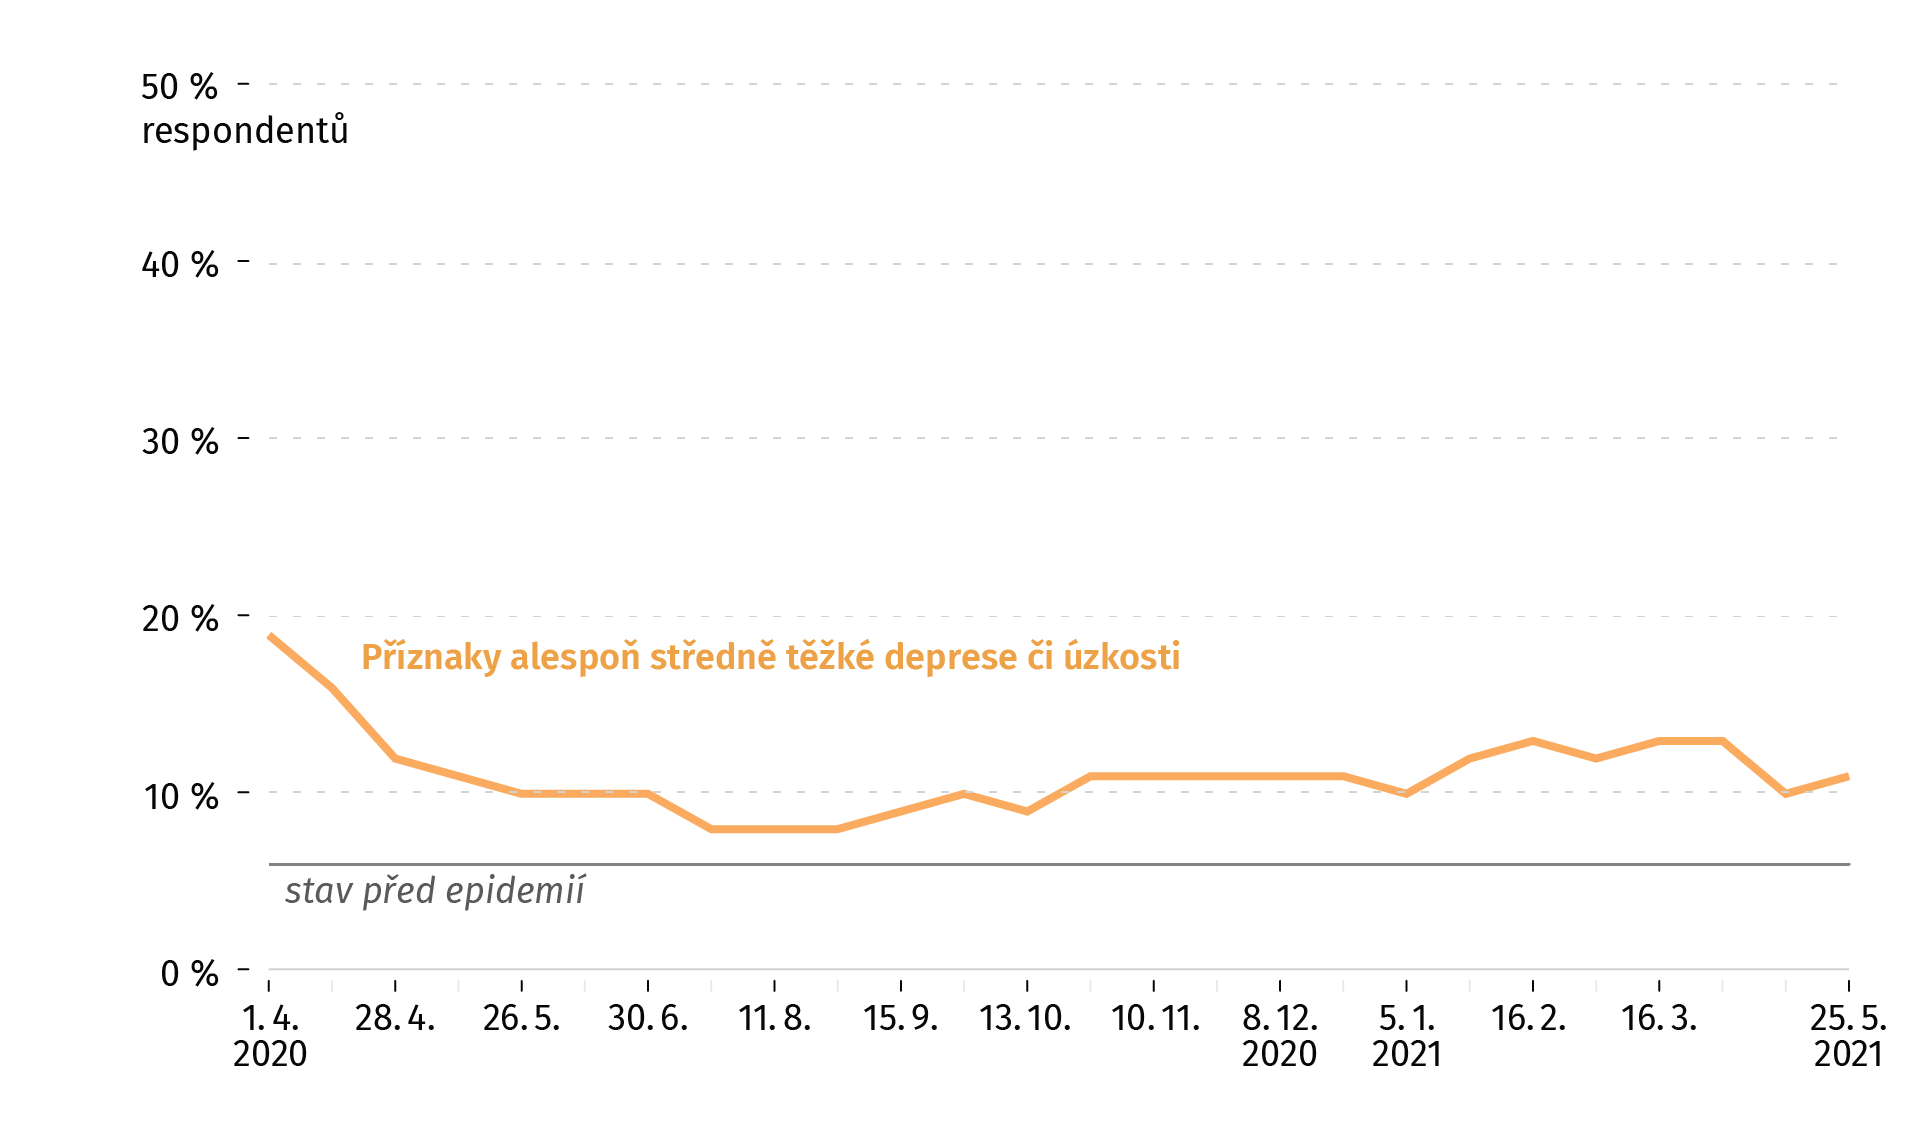
\includegraphics[width=\textwidth]{./pic/zbp-graf2.png}
    \caption{Zastoupení respondentů (18 a více let), kteří vykazují středně těžké příznaky deprese a úzkostí (podle zkrácené baterie PHQ8 a DAG7).}
    \label{fig:zbp2}
\end{figure}

Více informací a výsledky pro skupiny obyvatel viz: \url{https://zivotbehempandemie.cz/dusevni-zdravi}


\section*{Epidemiologicky klíčové proměny chování – sociální aktivity a chování}
\label{Epidemi_promeny}

% \subsection*{Sociální aktivity}
\label{Socialni_aktivity}

\paragraph{Sociální aktivity.} Vývoj reprodukčního čísla epidemie podle analýz BISOP vý\-raz\-ně závisí na tom, jak se vyvíjí reportovaný počet mezilidských kontaktů ve vý\-zku\-mu \uv{Život během pandemie}.\footnote{Viz analýzu BISOP z 22. února 2021
\url{https://www.bisop.eu/otazka-otazek-existuje-stale-nadeje-na-ucinne-a-relativne-rychle-reseni/}} A~počet těchto kontaktů naopak úzce souvisí se sociálními aktivitami, které se proměňovaly v závislosti na protiepidemických opatřeních, ale také v~souvislosti s~mírou obav a ochotou daná opatření dodržovat (compliance).

Výzkum \uv{Život během pandemie} sleduje celkem 13 aktivit, které se v~různých částech epidemie výrazně měnily. Hrubě je lze rozdělit na tři typy. Zaprvé volnočasové aktivity, které ve většině roku takřka vynulovaly přímé restrikce. Zadruhé rodinné aktivity a cestování, jejichž vývoj výrazně závisel na omezeních volného pohybu a~míře obav, a měnily se tedy plynuleji. A~zatřetí využívání služeb.

V~další volnočasové skupině činností je epidemiomologicky nezanedbatelnou aktivitou například návštěva restaurací. V~létě roku 2020 mezi první a druhou vlnou epidemie do nich týdně chodila téměř polovina respondentů. Při oficiálně zavřených restauracích zhruba 3~\% respondentů deklarovala, že do nich chodí. Toto číslo může být ovlivněno chybou (chybné zaškrtnutí v~dotazníku) i omezenou ochotou přiznat nedovolenou aktivitu. Ale celkově ukazuje, že zřejmě výrazně přeceňujeme vliv medializovaného porušování omezení služeb – jsou sice předmětem dílčího porušování, ale reálně dochází ke zhruba 95\% redukci jejich využívání i souvisejících kontaktů. Je vidět, že v~době mezi vlnami pandemie návštěvy restaurací stoupají postupně – zpočátku je ještě redukují obavy, jiný životní rytmus či zhoršená ekonomická situace respondentů a trvá 1,5 až 2 měsíce od otevření hospod, než se navrátí na původní intenzitu návštěv.

Ve druhé – sociální – skupině jsou klíčovou aktivitou návštěvy rodiny či přátel. V~první vlně na jaře 2020 došlo k~jejich velkému poklesu – s~rodinou a známými se stýkalo jen 33~\% respondentů. Postupně tato hodnota rostla až na 69~\%. V dalších vlnách epidemie
již nikdy lidé neomezili návštěvy jako na jaře 2020 – na vrcholu druhé vlny epidemie navštěvovalo rodinu či známé týdně 46~\%, ale již v~prosinci návštěvy velmi rostly. V~lednové třetí vlně návštěvy poklesly jen na 53~\% a na vrcholu 4. vlny ve druhém březnovém týdnu návštěvy přiznávalo 39~\% respondentů. Poslední vlna koronaviru se tím lišila od těch podzimních, což může být důsledek výraznějších obav, ale také většího omezení volného pohybu (přes hranice obcí a~okresů).

Využívání služeb se v rámci epidemie měnilo zřejmě nejméně. Vidíme výrazné proměny používání hromadné dopravy – v~prvním lockdownu roku 2020 MHD jezdilo jen 10~\% lidí, v létě mimo epidemii 33~\% a v~dalších fázích epidemie 20 až 30~\%. Kromě první vlny epidemie jsou ale výkyvy ve využívání hromadné dopravy spíše omezené. Data velmi silně korelují s~údaji o~mobilitě typu Public transport z přímého měření Google Mobility Report (GMR). Porovnání GMR napříč státy také ukazuje, že oproti například Portugalsku a Velké Británii, které v zimě 2021 také prošly výraznou vlnou viru varianty B-117 (tzv. britská varianta), klesla v~ČR mobilita daná využíváním veřejné dopravy méně. To je dáno mimo jiné tím, že využívání veřejné dopravy výrazně souvisí s dojížděním do práce. A~právě omezené využívání home office je jedním ze specifik epidemie v ČR.

\begin{figure}[ht]
    \centering
    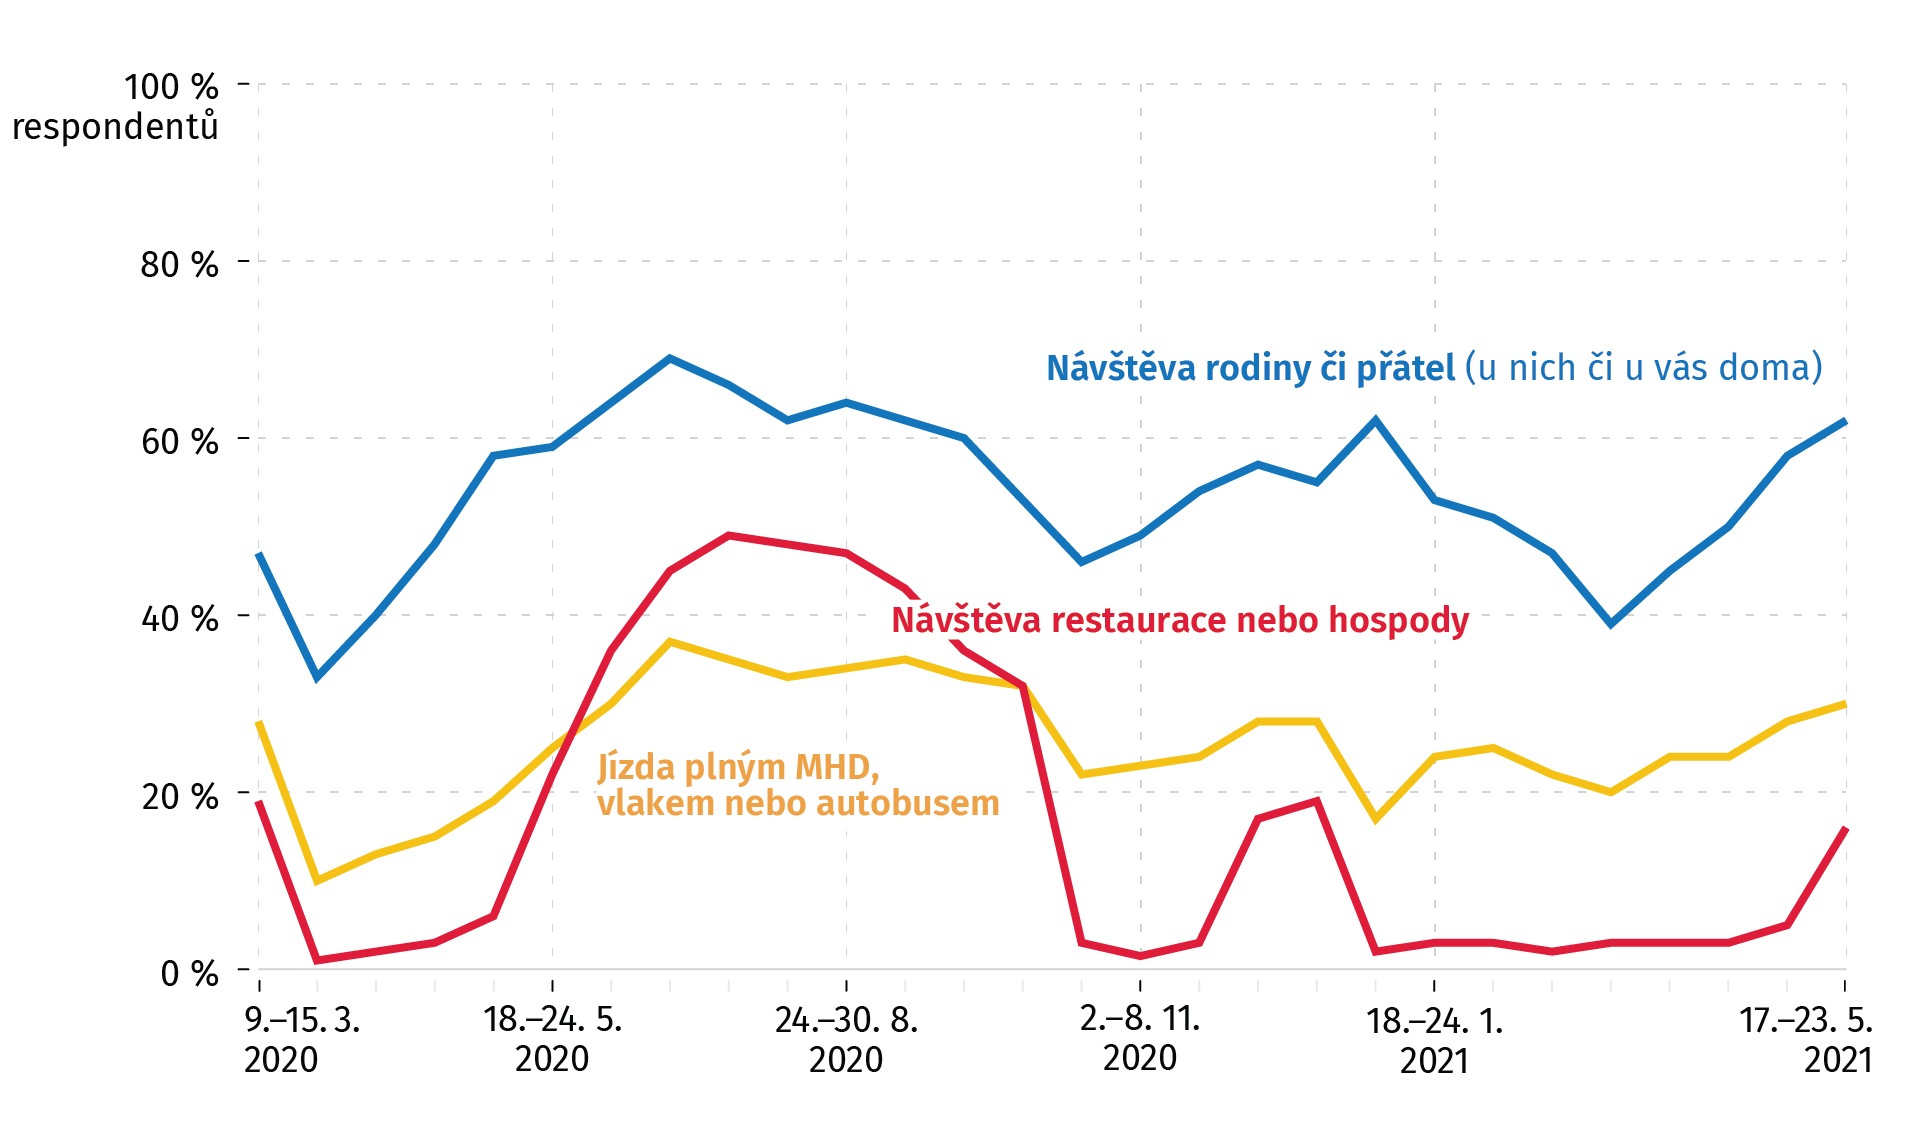
\includegraphics[width=\textwidth]{./pic/zbp-graf3.png}
    \caption{Zastoupení respondentů (18 a více let), kteří v daném týdnu alespoň 1x vykonávali danou aktivitu.}
    \label{fig:zbp3}
\end{figure}


Více informací a výsledky pro skupiny obyvatel jsou uvedeny na WWW stránkách: \url{https://zivotbehempandemie.cz/socialni-aktivity}


%\subsection*{Využívání home office}

\paragraph{Využívání home office.} Osobní přítomnost v práci v průměru až dvojnásobně rozšiřuje okruh osob, s nimiž lidé přicházejí do blízkého kontaktu (viz oddíl Ekonomické dopady na domácnosti na straně \pageref{Ekonomicke_dopady}). Podrobnější analýzy provedené tzv. regresními stromy na prvních 20 vlnách výzkumu \uv{Život během pandemie} přitom ukazují, že v ČR do práce chodilo 53\,\% respondentů, kteří měli typické příznaky (ztráta čichu/chuti a teplota) a neměli pozitivní test, a okolo 70\,\% těch, kteří byli v kontaktu s někým nakaženým a byli bez příznaků. I~pracovní kolektivy tedy byly zřejmě důležitým místem přenosu, což naznačují i data z trasování zveřejněná Ústavem zdravotnických informací a statistiky (ÚZIS).\footnote{Viz prezentaci Ladislava Duška (UZIS) 19. února 2021 v~Poslanecké sněmovně Parlamentu ČR \url{https://drive.google.com/file/d/1rEaXGTexjmKZu2MUJGc6thr0RtZaWBJi/view}} Jednou z velkých otázek epidemie tak je, jak přítomnost lidí na pracovištích omezit – mimo využívání nemocenské a karantén také využitím home office u~ostatních pracovníků.

Podle studií Eurofondu v zemích západní Evropy a Skandinávie v době nejvyššího výskytu koronaviru pracovalo z domova 40 až 50\,\% lidí.\footnote{ \url{https://www.eurofound.europa.eu/publications/report/2020/living-working-and-covid-19}} Tyto trendy výrazného poklesu přítomnosti na pracovištích potvrzuje i Google Mobility Report (viz Sociální aktivity na straně \pageref{Socialni_aktivity}). V České republice, kde 37\,\% lidí pracuje v průmyslu, je možnost home office omezená. Podle odhadů think-tanku IDEA ze struktury pracovního trhu může v~režimu home office v ČR pracovat zhruba každý třetí za\-měst\-na\-nec.\footnote{\url{https://idea.cerge-ei.cz/files/IDEA\_Home\_office\_covid-19\_rijen\_23\_2020/files/basic-html/page1.html}} Tomu odpovídá fakt, že v rámci výzkumu \uv{Život během pandemie} více než 30\,\% pracovně aktivních lidí alespoň dva týdny v roce 2020 pracovalo z domova. Ani tento omezený potenciál home office nebyl v některých fázích epidemie plně vytěžen.

Lockdown na jaře 2020 dostal velkou část pracujících (zaměstnanců a OSVČ) do dočasné neaktivity z důvodu nucené dovolené, ošetřovného, nemocenské, omezení práce zaměstnavatelem či z~dalších příčin. Přibližně pětina pracujících od poloviny března do poloviny května uváděla, že v~předchozím týdnu nevykonávala svoji práci. Současně řada lidí přešla na práci z domova. Navíc 22\,\% pracujících pracovalo na plný home office a 11\,\% chodilo na pracoviště jen částečně. Výsledkem bylo, že od března do poloviny května se na pracovišti plně vyskytovala méně než polovina pracovně aktivních Češek a Čechů (46\,\%).

K takovému omezení přítomnosti na pracovišti už nikdy v dalších vlnách epidemie nedošlo. V~podzimní druhé vlně epidemie využívalo plně home office maximálně 16\,\% pracujících a přes 60\,\% chodilo na pracoviště. K~výraznému rozšíření koronaviru v lednu a únoru 2021 mohlo přispět to, že v těchto měsících využívání plného home office dále pokleslo na 13\,\% a podíl lidí docházejících plně na pracoviště stoupl na dvě třetiny. V zatím poslední vlně epidemie na jaře 2021, kdy byl psán tento text, naopak Češi omezili přítomnost na pracovištích více a zejména na delší dobu než na podzim předchozího roku.

Během celé epidemie je práce z domova nejvíce rozšířena v odvětví IT a financí. Výrazně omezená byla po celou dobu epidemie ve státní správě, ale také v odvětvích služeb, průmyslu a zemědělství. Nevyužívání home office má důvody v neochotě zaměstnanců, ale i firem. V ad hoc otázkách v březnu 2020 odpovědělo 16\,\% pracujících, že jim zaměstnavatel někdy v uplynulých měsících nedovoloval pracovat z domova, ačkoli to bylo možné.

\begin{figure}[ht]
    \centering
    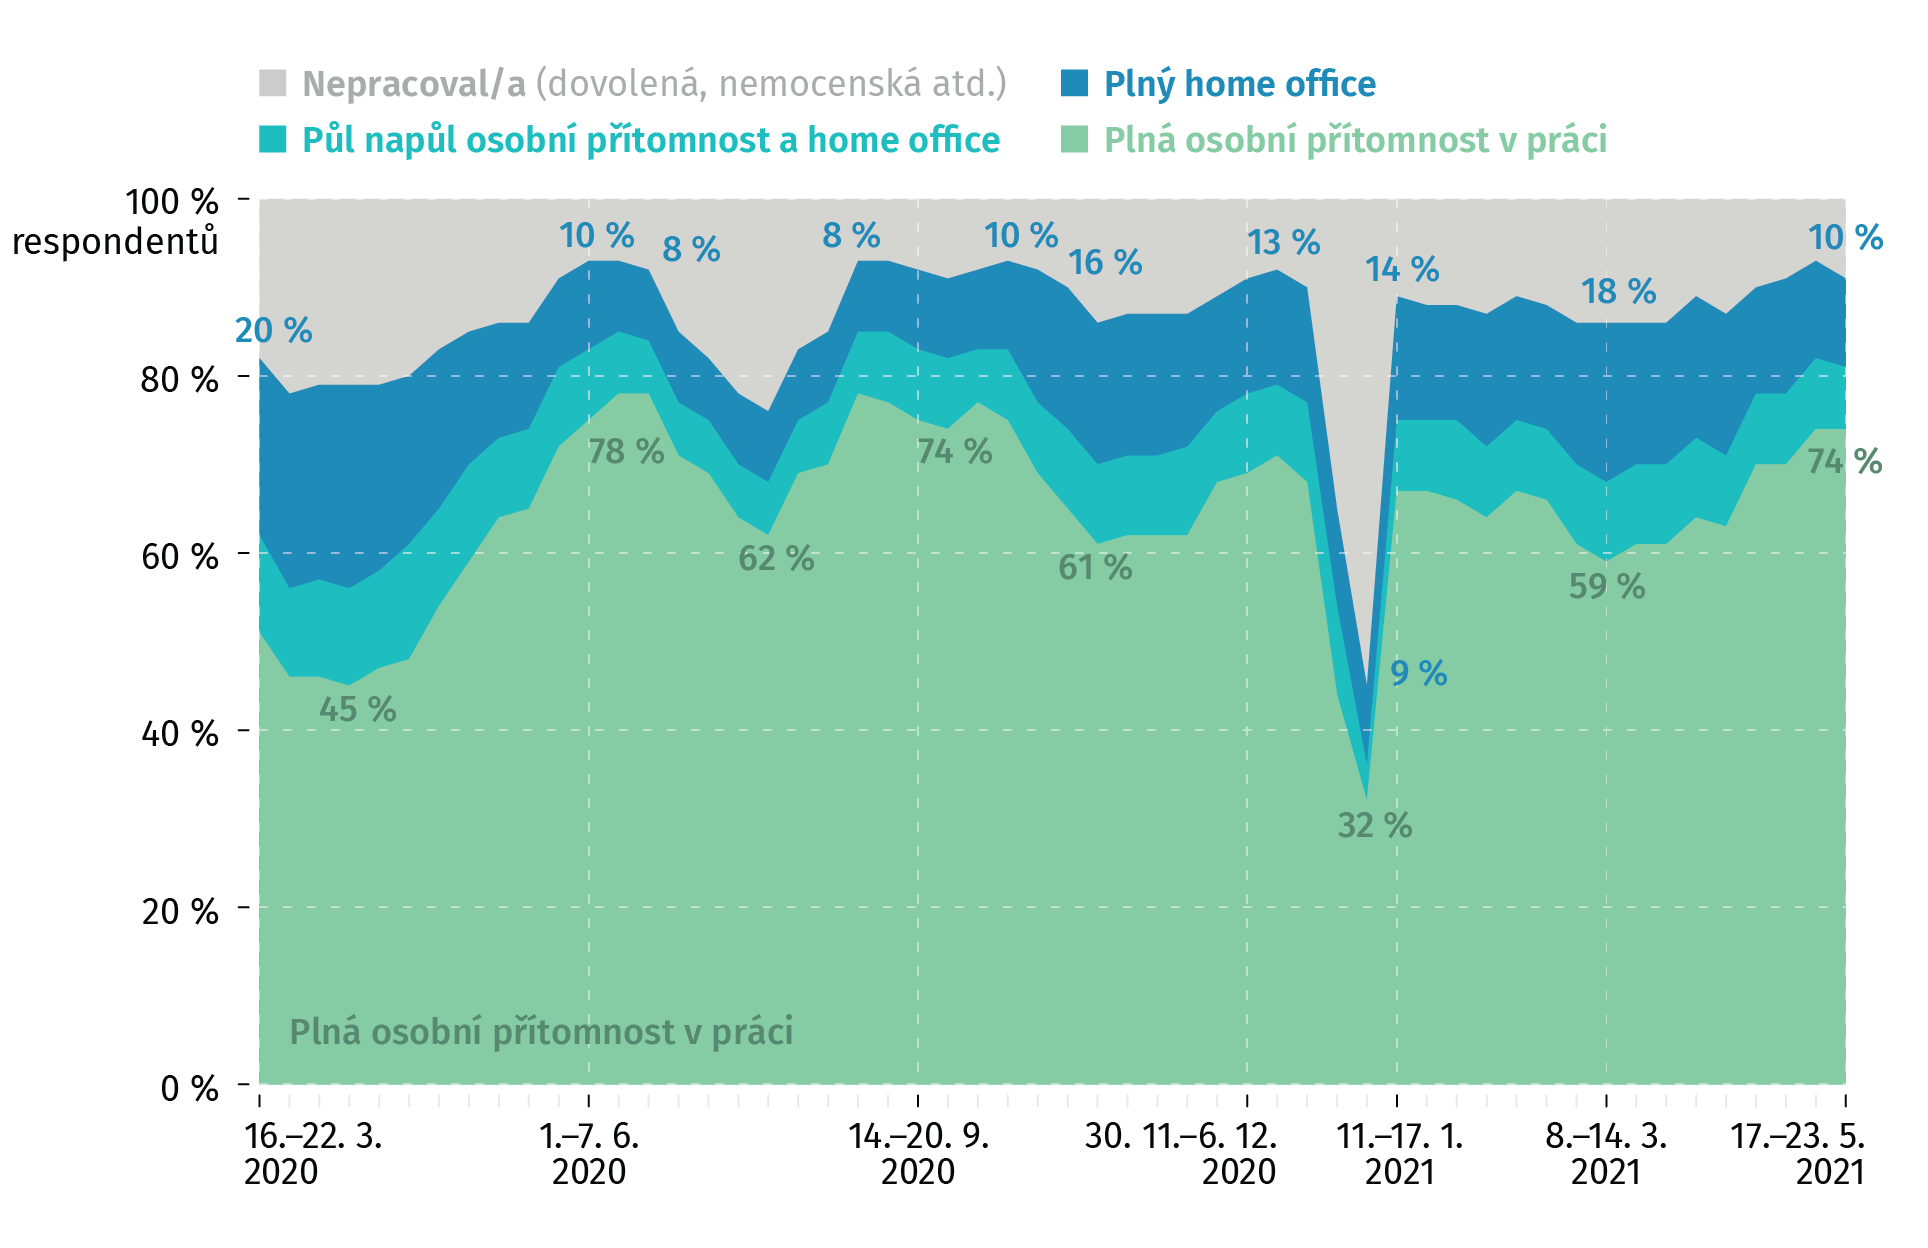
\includegraphics[width=\textwidth]{./pic/zbp-graf4.png}
    \caption{Vývoj využívání home office a přítomnosti na pracovišti (pracovně aktivní populace).}
    \label{fig:zbp4}
\end{figure}

Více informací a výsledky pro skupiny obyvatel viz \url{https://zivotbehempandemie.cz/home-office}.

\section*{Vývoj kontaktů: Na čem záleží a jak lze predikovat}

Po shrnutí některých základních trendů v chování a sociálních aktivitách se nabízí otázka, jak vlastně tyto aktivity ovlivňují míru kontaktů, které úzce souvisejí s tzv. reprodukčním číslem a šířením epidemie (viz Epidemiologicky klíčové proměny cho\-vá\-ní – sociální aktivity a chování na straně \pageref{Epidemi_promeny}). 

Z veřejných dat výzkumu \uv{Život během pandemie} víme, že průměrný reportovaný počet lidí, s nimiž jsou respondenti v osobním kontaktu alespoň pět minut, se pohyboval okolo 24 v době mimo epidemii (léto 2020). V prvním lockdownu na jaře 2020 klesl na průměr sedm až osm kontaktů. V podzimní vlně epidemie se minimum pohybovalo okolo 13 kontaktů a na jaře 2021 pokleslo na 10--11 kontaktů, ale nikdy se nedostalo na úroveň jara 2020. Míra kontaktů různých respondentů se výrazně liší – podle typu jejich domácnosti, věku, socioekonomického statusu a typu práce i podle volnočasových aktivit. U~různých respondentů se však také výrazně jinak vyvíjela s ohledem na epidemickou situaci a platné restrikce. Kde se ale v různých dobách epidemie vlastně mezilidské kontakty odehrávaly a jaký vliv kvůli tomu mohly mít aditivní restrikce a společenská omezení? 

Modelování na 28 vlnách dat výzkumu \uv{Život během pandemie} ukazuje, že na\-pří\-klad přestat chodit do práce má relativně velký efekt na počet kontaktů – prů\-měr\-né\-mu respondentovi v takovém případě v daném týdnu ubude okolo 15 osobních kontaktů. A~to při kontrole změny ostatních aktivit, sociodemografie a celkové společenské situace v dané době (viz Metodika). Tyto efekty ukazuje druhý sloupec tabulky \ref{tab:narust-kontaktu} regresního modelu níže. Třetí sloupec ukazuje, jak velké části společnosti se dané aktivity týkají – a to v létě 2020 (23. týden)
v době bez spo\-le\-čen\-ských restrikcí. V~této době chodilo do práce 47,5\,\% respondentů, ostatní byli pracovně neaktivní, nepracovali či byli na home office. 


\begin{table}[ht]
    \centering
    \caption{Nárůst kontaktů při dané aktivitě v průměrném týdnu u~průměrného respondenta (model)}
    
\begin{tabular}{ p{5cm} p{2cm} p{2cm} p{2cm}  }
 \hline
 Aktivity & Beta \newline (efekt na \newline nárůst kontaktů) & Směrodatná \newline chyba & Zásah populace \newline 23. týden (\%)\\
 \hline
 Konstanta   & 2,3    & & \\
 Návštěva práce (či VŠ) & 15,0 & 0,7 &47,5\\
 Návštěva větších sportovních utkání či kulturních akcí ($>$ 500 účastníků) &
6,3 &
0,6 &
3,8\\
  Návštěva menších sportovních utkání či kulturních akcí ($<$ 500 účastníků)&
4,2&
0,4&
10,1\\
  Účast na společenské události za přítomnosti více než pěti lidí (např. svatba)&
3,6&
0,3&
11,4\\
  Společná dovolená či výlet s~více lidmi&
3,1&
0,2&
15,8\\
  Návštěva restaurace nebo hospody&
3,0&
0,2&
46,5\\
  Využití veřejných toalet&
2,8&
0,2&
25,2\\
  Jízda plným MHD, vlakem nebo autobusem&
1,8&
0,1&
46,8\\
  Návštěva fitness, sportovišť, hraní týmových sportů&
1,4&
0,3&
11,2\\
  Chození do parku, po městě apod. ve více než dvou lidech&
1,0&
0,1&
33,7\\
  Návštěva rodiny či přátel (u~nich či u~vás doma)&
0,9&
0,1&
65,4\\
  Nakupování v~obchodě (popř. návštěva banky/pošty) s~větším množstvím lidí&
0,7&
0,1&
84,9\\
 \hline
\end{tabular}
    
    \label{tab:narust-kontaktu}
\end{table}

Pozn.: V tabulce \ref{tab:narust-kontaktu} jsou uvedeny jen aktivity, u~nichž lze díky velikosti smě\-ro\-dat\-né chyby říct, že s~95\% spolehlivostí vedou k navýšení mezilidských kontaktů.

\vspace{1em}
\paragraph{Metodika.} Lineární regresní model na datech 1.--28. vlny výzkumu \uv{Život během pandemie} (březen 2020–květen 2021). Jednotkou analýzy jsou respondento-týdny. Predikovaná proměnná: počet odhadovaných osobních kontaktů delších než 5 minut. Model tak odhaduje vliv aktivit a jejich změn na změnu kontaktů.

Kontrolována je vedle sociodemografických údajů (věk, velikost domácnosti, pohlaví, velikost obce, vzdělání) také míra obav odpovídající celkové míře restrikcí ve společnosti při daném scénáři celkové sumy aktivit, tak aby regresní model ukazoval přímé efekty aktivit, nikoli jejich nepřímou souvislost s počtem kontaktů kvůli tomu, že při zákazu a omezení aktivit narůstá i míra obav z epidemie.

U~většiny aktivit předpokládáme tzv. fixed effect, stejné efekty u~všech respondentů – tedy, že například návštěva restaurace přidává všem respondentům zhruba stejný počet kontaktů. U některých aktivit se však reálné efekty výrazně liší mezi respondenty – například návštěva práce má různý efekt podle toho, kde respondent pracuje. U~těchto aktivit předpokládáme individuálně proměnlivé efekty (beta) a~v tabulce výše je zobrazen průměr za respondenty ve výzkumu.

Model prošel testem dobré shody. Proběhlo porovnání skutečně reportovaných kontaktů a predikovaných kontaktů, model má dobrý fit v celém průběhu epidemie, který navíc existuje v rámci různých skupin obyvatel – například mezi kvartily respondentů podle výchozí úrovně kontaktů mimo epidemii.
\vspace{1em}

\noindent Zcela jinou strukturu dopadů na kontakty má například omezení návštěv přátel a rodiny. To přidává v průměru jen necelý jeden kontakt (0,9). Kontakty jsou ve výzkumu definovány jako počet lidí, se kterými byl respondent v daném týdnu alespoň 5 minut fyzicky v kontaktu. Je tedy možné, že s některými příbuznými či přáteli, s nimiž se respondenti navštěvují, jsou v kontaktu i v práci, což omezuje přidaný efekt návštěv. Rodinu a přátele však, mimo epidemii, navštěvují 2/3 lidí. V nejtvrdších lockdownech toto číslo kleslo na 1/3. Omezení návštěv tedy redukuje méně kontaktů, ale u~daleko vyššího procenta populace. Zároveň se tyto kontakty odehrávají často bez roušek a trvají nad 15 minut. 

Restaurace také patří mezi aktivity, které mají omezený efekt na kontakty – jejich návštěva většinou rozšiřuje odhadovaný sociální okruh v průměru o~tři lidi a významné kontakty s nimi – ale týkají se 46\,\% lidí, kteří do restaurací chodí i v době mimo epidemii. 

Je nutno poznamenat, že z vlivu aktivit na kontakty nelze přímo odvodit jejich epidemiologickou důležitost. Kontakty při návštěvách a v práci často trvají déle, ale mohou být jinak chráněny. Kontakty v restauracích mohou probíhat na zahrádkách i ve vnitřních prostorách, kde problém nepředstavuje počet lidí v přímém kontaktu při komunikaci, ale také aerosoly setrvávající ve vzduchu. To se týká i jiných prostředí (MHD). 

Z modelu však vyplývá minimálně to, že neexistuje „zázračné“ řešení, které by mezilidské kontakty dospělé populace eliminovalo pomocí jednoho či dvou ne\-ná\-roč\-ných opatření. Uzavření restaurací a výrazné omezení všech volnočasových aktivit kontakty redukuje, ale velká část se odehrává v práci, v rodinách a na návštěvách. Tedy v lokacích, kde podle Ústavu zdravotnických informací a statistiky (ÚZIS) také často docházelo k šíření viru.

S využitím modelu můžeme odhadnout, jak by se průměrný počet kontaktů vyvíjel, pokud by se v různých obdobích epidemie aplikovaly další restrikce aktivit. Viz obrázek \ref{fig:zbp5}. Červená linie ukazuje skutečný stav kontaktů vzhledem k existujícím aktivitám. Druhá linie zobrazuje odhadovaný stav kontaktů, pokud by se striktně uplatnily a vymáhaly restrikce, které platily po většinu podzimu a celou zimu až do 28. února 2021. Vidíme, že by logicky snížily počet kontaktů v letních měsících – protože v té době by přidaly omezení. Restrikce však vedly k dílčímu omezení i v době, kdy platily, protože část kontaktů probíhala v neoficiálně otevřených restauracích a při jiných nepovolených aktivitách, které respondenti přiznávali. Tento vliv je však podle modelu relativně malý. 

Třetí linie grafu ukazuje, že k dalšímu omezení o~1 až 1,5 kontaktu u~průměrného Čecha nad 15 let by vedla maximalizace home office. To vyplývá z faktu, že home office redukuje u člověka 15 kontaktů, ale potenciál jeho navýšení se pohyboval jen mezi 8--10\,\% dospělé populace. Předposlední, fialová linie grafu ukazuje, že úplná redukce návštěv, cestování a volnočasových aktivit by v různých obdobích redukovala další významný počet kontaktů. Je však vidět, že i při tomto společensky extrémně nákladném scénáři, který výrazně omezí kvalitu života, je míra kontaktů relativně vysoká. Uplatnění těchto opatření navíc není realistické, protože předpokládá dodržování těžko vymahatelných pravidel. I kdyby se ve 4. vlně epidemie v březnu 2021 bylo podařilo tyto restrikce uplatnit, míra kontaktů by stejně neklesla na úroveň kontaktů z prvního lockdownu (březen--duben 2021), kdy byl klíčový rozdíl v tom, že na pracoviště chodilo méně lidí. A~právě v redukci kontaktů na pracovišti byl podle naší analýzy další velký potenciál redukce kontaktů – teoreticky o~dalších zhruba pět kontaktů v průměru (viz poslední, oranžovou linii). To by však předpokládalo úplný lockdown s uzavřením majority pracovišť, tedy ekonomicky velmi nákladné řešení, jehož alternativou je snaha o maximální bezpečnost na pracovištích – testování a zvýšení využívání karantén a~izolací rizikových pracovníků.

\begin{figure}[ht]
    \centering
    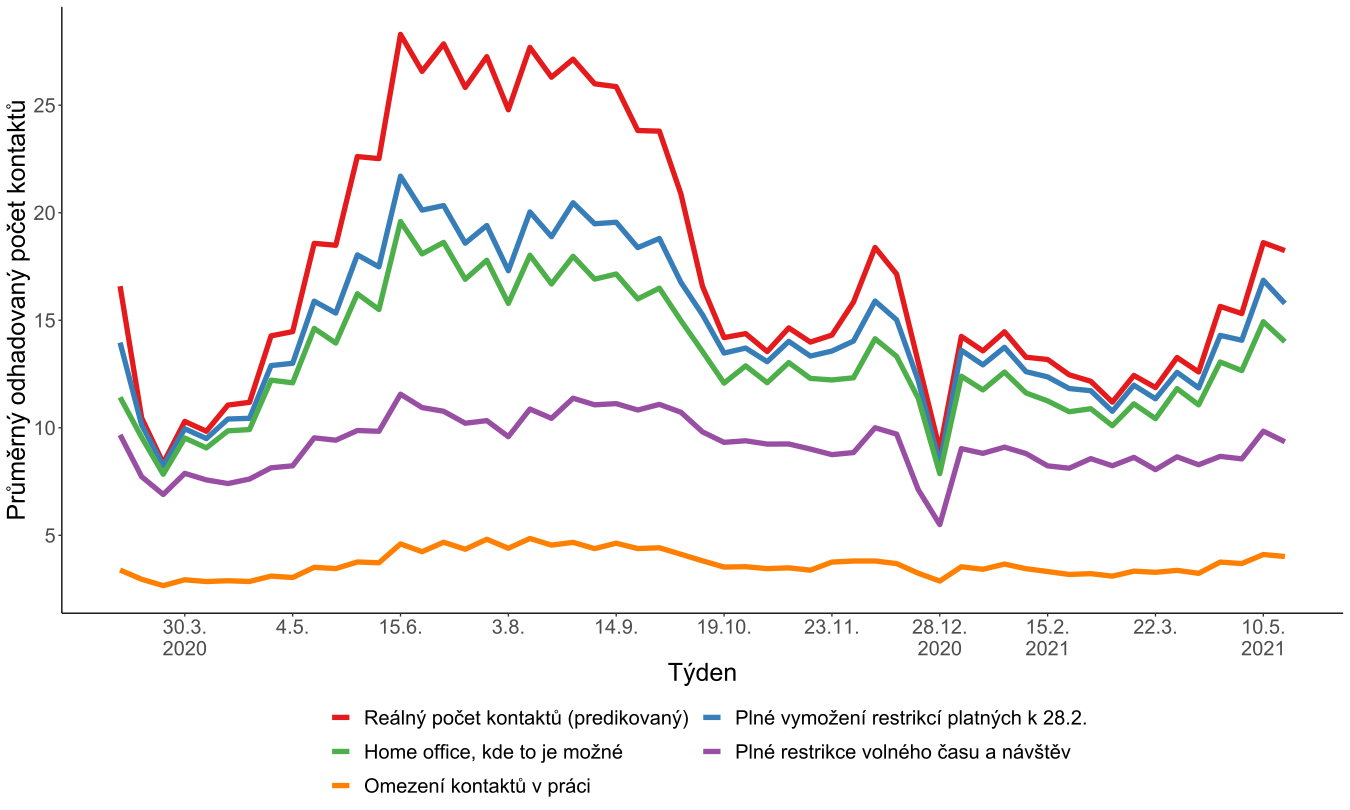
\includegraphics[width=0.95\textwidth]{./pic/zbp-graf5.png}
    \caption{Průměrný odhadovaný počet kontaktů při různých scénářích restrikcí.}
    \label{fig:zbp5}
\end{figure}


\section*{Obrana před epidemií: Očkování a testování}

Ke dvěma formám obrany před epidemií, které nevedou cestou restrikce aktivit s velkým dopadem na ekonomiku a well-being obyvatel, patří očkování a správná strategie testování. Respondenti \uv{Života během pandemie} byli poprvé dotazováni na zájem o~očkování koncem září, kdy ochotu nechat se zdarma naočkovat proti nemoci covid-19 projevilo 56\,\% dospělých. Následně v rámci stejného panelu respondentů došlo k propadu ochoty, který podle dat souvisel s nárůstem obav z vedlejších účinků vakcín, ale i s nárůstem velmi kritického postoje k institucím a řešení epidemie. Od začátku roku 2021 však ochota k očkování stoupala. Na konci května 2021 souhlas projevily dvě třetiny dospělých (67\,\%), z nichž přibližně 43\,\% již dostalo alespoň jednu dávku vakcíny. 

Za pozitivním trendem se však skrývají dva odlišné příběhy. Na jedné straně je to vysoký a rostoucí zájem mezi lidmi nad 55 let a lidmi s vyšším vzděláním, který mezi zářím 2020 a květnem 2021 vzrostl z hodnot pod 60\,\% na více než 80\,\%. Na druhé straně je to velmi omezený zájem mezi lidmi do 54 let bez maturity a z menších obcí i mezi lidmi z~chudších domácností. U této skupiny došlo k velkému propadu ochoty a důvěry k vakcinaci na podzim roku 2020 a přes mírný nárůst se od té doby nikdy nedostala výrazně nad 50\,\%. 

Problematické pro budoucnost „kolektivní imunity“ je také to, že menší zájem výzkum eviduje u~osob, které se méně chrání před nákazou nebo jejím přenosem. Jde právě o~mladší lidi s nižším vzděláním a z menších obcí. Existuje tedy riziko, že nevakcinovaná zůstane skupina, která sice nepatří mezi zdravotně nejrizikovější, ale může se výrazně podílet na dalším šíření viru a jeho nových variant.

\begin{figure}[ht]
    \centering
    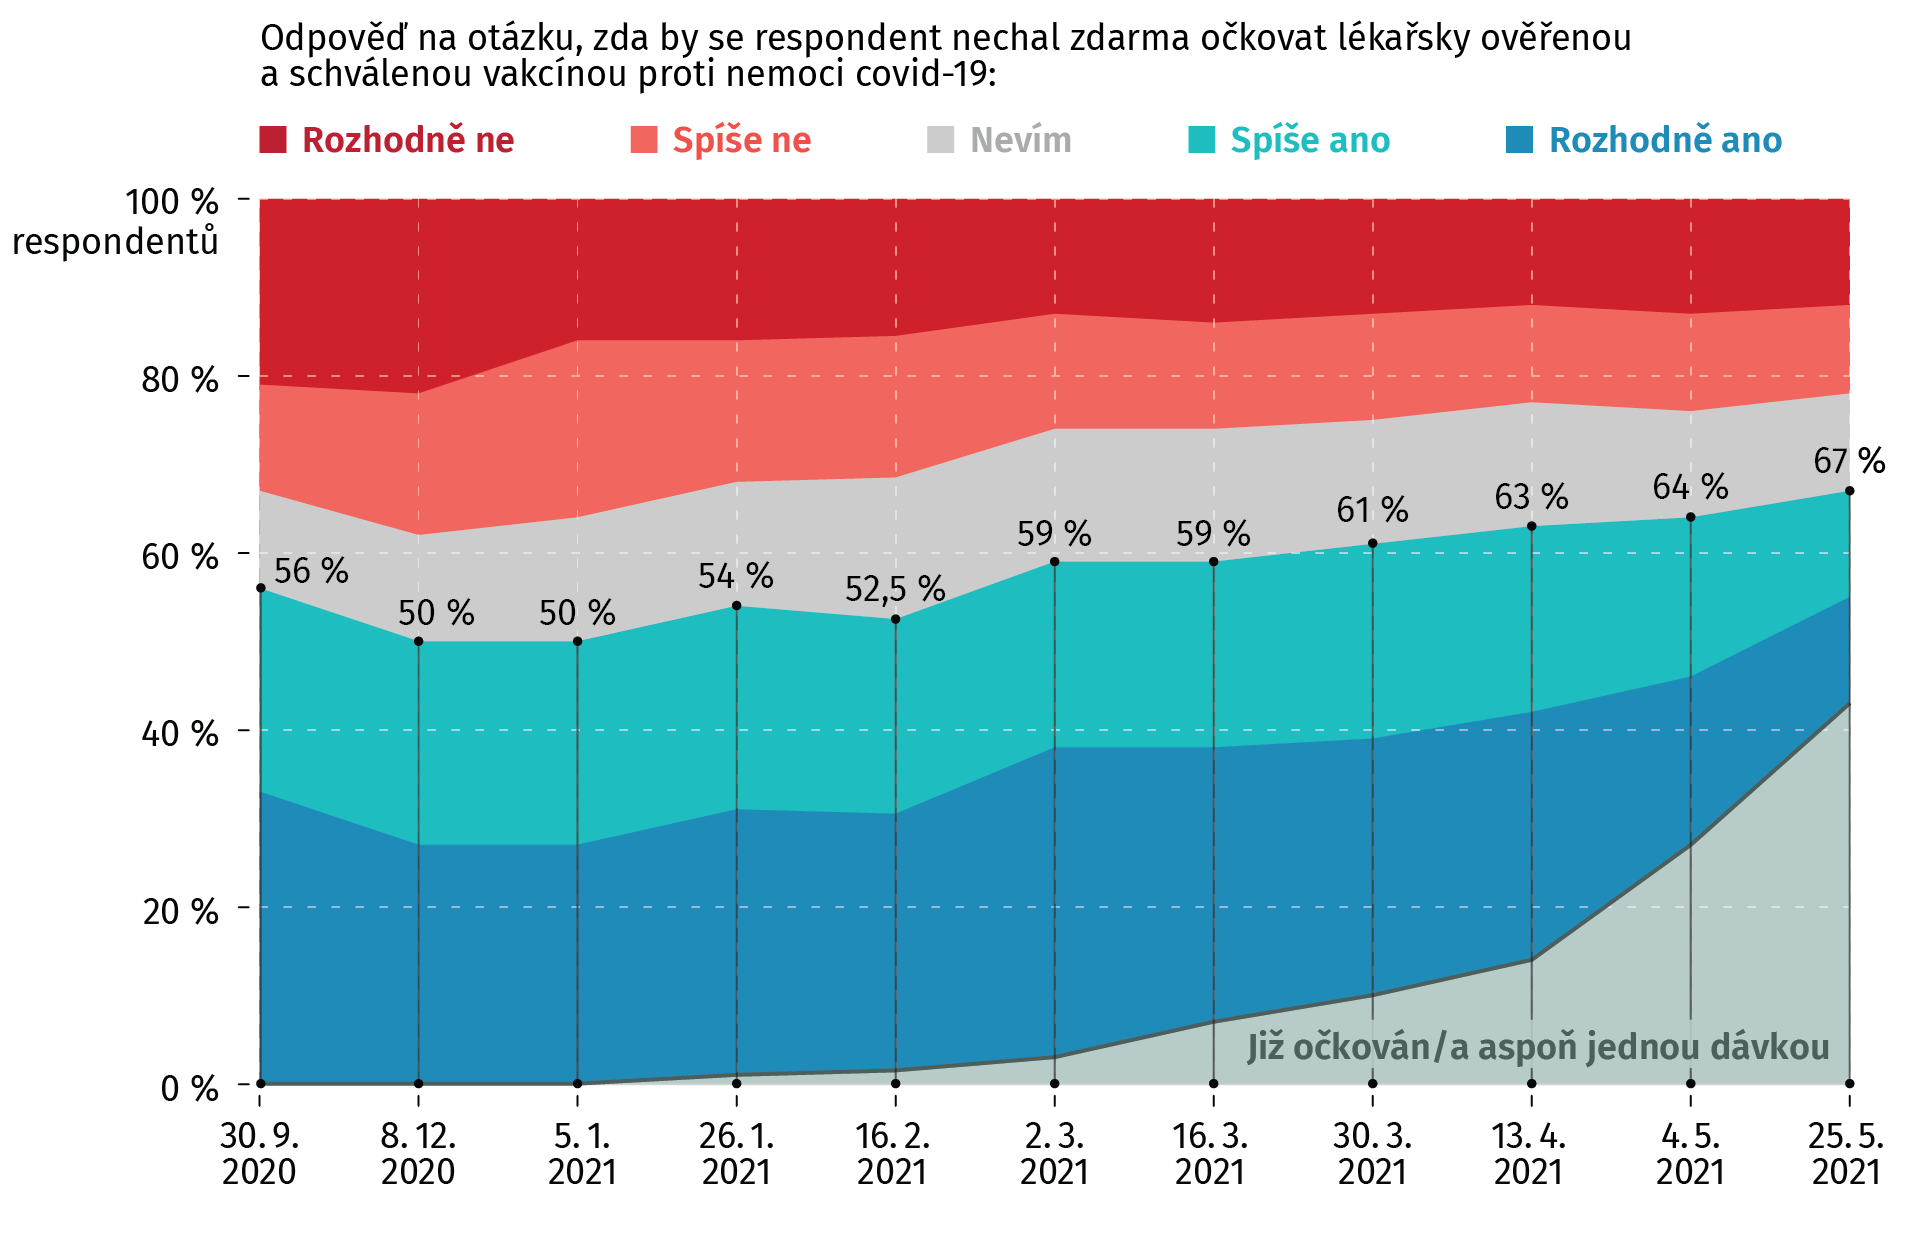
\includegraphics[width=0.95\textwidth]{./pic/zbp-graf6.png}
    \caption{Vývoj ochoty k očkování včetně již očkovaných (respondenti 18 a více let).}
    \label{fig:zbp6}
\end{figure}

Více informací a výsledky pro skupiny obyvatel viz: \url{https://zivotbehempandemie.cz/ockovani}

Kromě výrazně zrychlené vakcinace v březnu až květnu 2021 ke „zkrocení“ epidemie přispělo posílení testování. Z oficiálních dat ÚZIS sice víme, kolik lidí je testováno a s jakou mírou pozitivity, ale nevíme, kolik nakažených lidí testováním neprochází. To lze hrubě odhadovat z příjmů v nemocnicích (zda se lidé dovídají o~koronaviru až tam), ale také z výzkumu \uv{Život během pandemie}. 

Ten ukazuje kritickou situaci na podzim roku 2020. Z respondentů, kteří v posledním měsíci byli v kontaktu s nakaženým či pociťovali typické příznaky koronaviru (ztráta čichu/chuti), procházelo testováním jen okolo 30\,\%. Konkrétně v týdnu do 10. listopadu bylo 12\,\% respondentů takto rizikových a neprošlo testem, zatímco jen 6\,\% rizikových testem prošlo. Tento stav se začal měnit až v lednu a definitivně pak v průběhu března a dubna 2021, kdy naopak okolo 60\,\% rizikových lidí procházelo nějakým typem testu. To je mj. pozitivní důsledek
povinného testování ve firmách, jenž byl vidět i v mírném poklesu počtu hospitalizovaných, kteří se o~nemoci dověděli až při příjmu, a v tom, že podle predikce Svazu průmyslu a dopravy testování ve firmách odhalilo měsíčně minimálně 60--65 tisíc případů pouze v průmyslu. Ve skutečnosti však může být projekce zahrnující všechny zaměstnavatele i výrazně vyšší.\footnote{Svaz průmyslu a dopravy České republiky uvedl, že při projekci z míry odhalení v jeho firmách na všechny zaměstnavatele průmyslu odhaduje 50 tisíc odhalených případů covid-19 ve třech týdnech měsíce března – tedy minimálně 60--65 tisíc za měsíc. Svaz průmyslu a dopravy ovšem sdružuje spíše odpovědné zaměstnavatele, z nichž řada investovala do opatření a testování již před povinností. Reálná míra odhalení antigenními testy v celém průmyslu tedy může být vyšší a zároveň průmysl je jen částí zaměstnavatelů, kteří museli testovat. \url{https://www.spcr.cz/pro-media/tiskove-zpravy/14483-testovani-na-covid-19-ve-firmach-funguje-podil-pozitivnich-testu-klesa}}

\section*{Imunizace jako faktor vývoje kontaktů}

Zrychlené očkování na jaře 2021 a také fakt, že onemocněním covid-19 prošla velká část populace, vedly k postupnému nárůstu imunizace. Výzkum \uv{Život během pandemie} ukazuje, že skupina očkovaných se částečně překrývá s lidmi, kteří nemocí v minulosti prošli. Alespoň částečnou prokazatelnou imunitu mělo ke konci května 51\,\% respondentů – 43\,\% mělo alespoň jednu dávku vakcíny, ale navíc 8\,\% prodělalo covid-19 v posledních šesti měsících. Tato forma imunity není úplná a dostatečná, ale na druhou stranu lze odhadovat, že další část respondentů nemoc měla, ale nebyla testována.

Počet respondentů, kteří jsou prokazatelně alespoň částečně imunní, začal výrazně růst až v průběhu dubna 2021. Míra imunizace ovlivňuje epidemiologický význam zmiňovaných osobních kontaktů. Tento vývoj ilustruje odhad počtu kontaktů, při nichž ani jedna ze stran nemá ani částečnou prokazatelnou imunitu.\footnote{V tomto odhadu zohledňujeme, zda je respondent očkovaný či nemoc prodělal v~posledním půlroce, a u neimunních respondentů počítáme s tím, že alespoň částečnou imunitu má takové procento jeho kontaktů, které odpovídá zastoupení částečně imunizovaných v celé populaci. Tato míra je ilustrativní, protože imunita daná jednou dávkou či proděláním nemoci před více měsíci není úplná. Na druhou stranu nezohledňuje ani to, že část respondentů nebyla testována, a tak nevědí o~tom, zda covid-19 měli.} Počet těchto kontaktů se od prostého průměru kontaktů začal výrazně oddělovat právě na konci března a začátku dubna. Ke konci května se průměrný počet kontaktů, při nichž ani jedna strana nemá ani částečnou imunitu, pohyboval okolo pěti až šesti, ačkoli prostý průměr kontaktů opět stoupal nad patnáct.

\begin{figure}[ht]
    \centering
    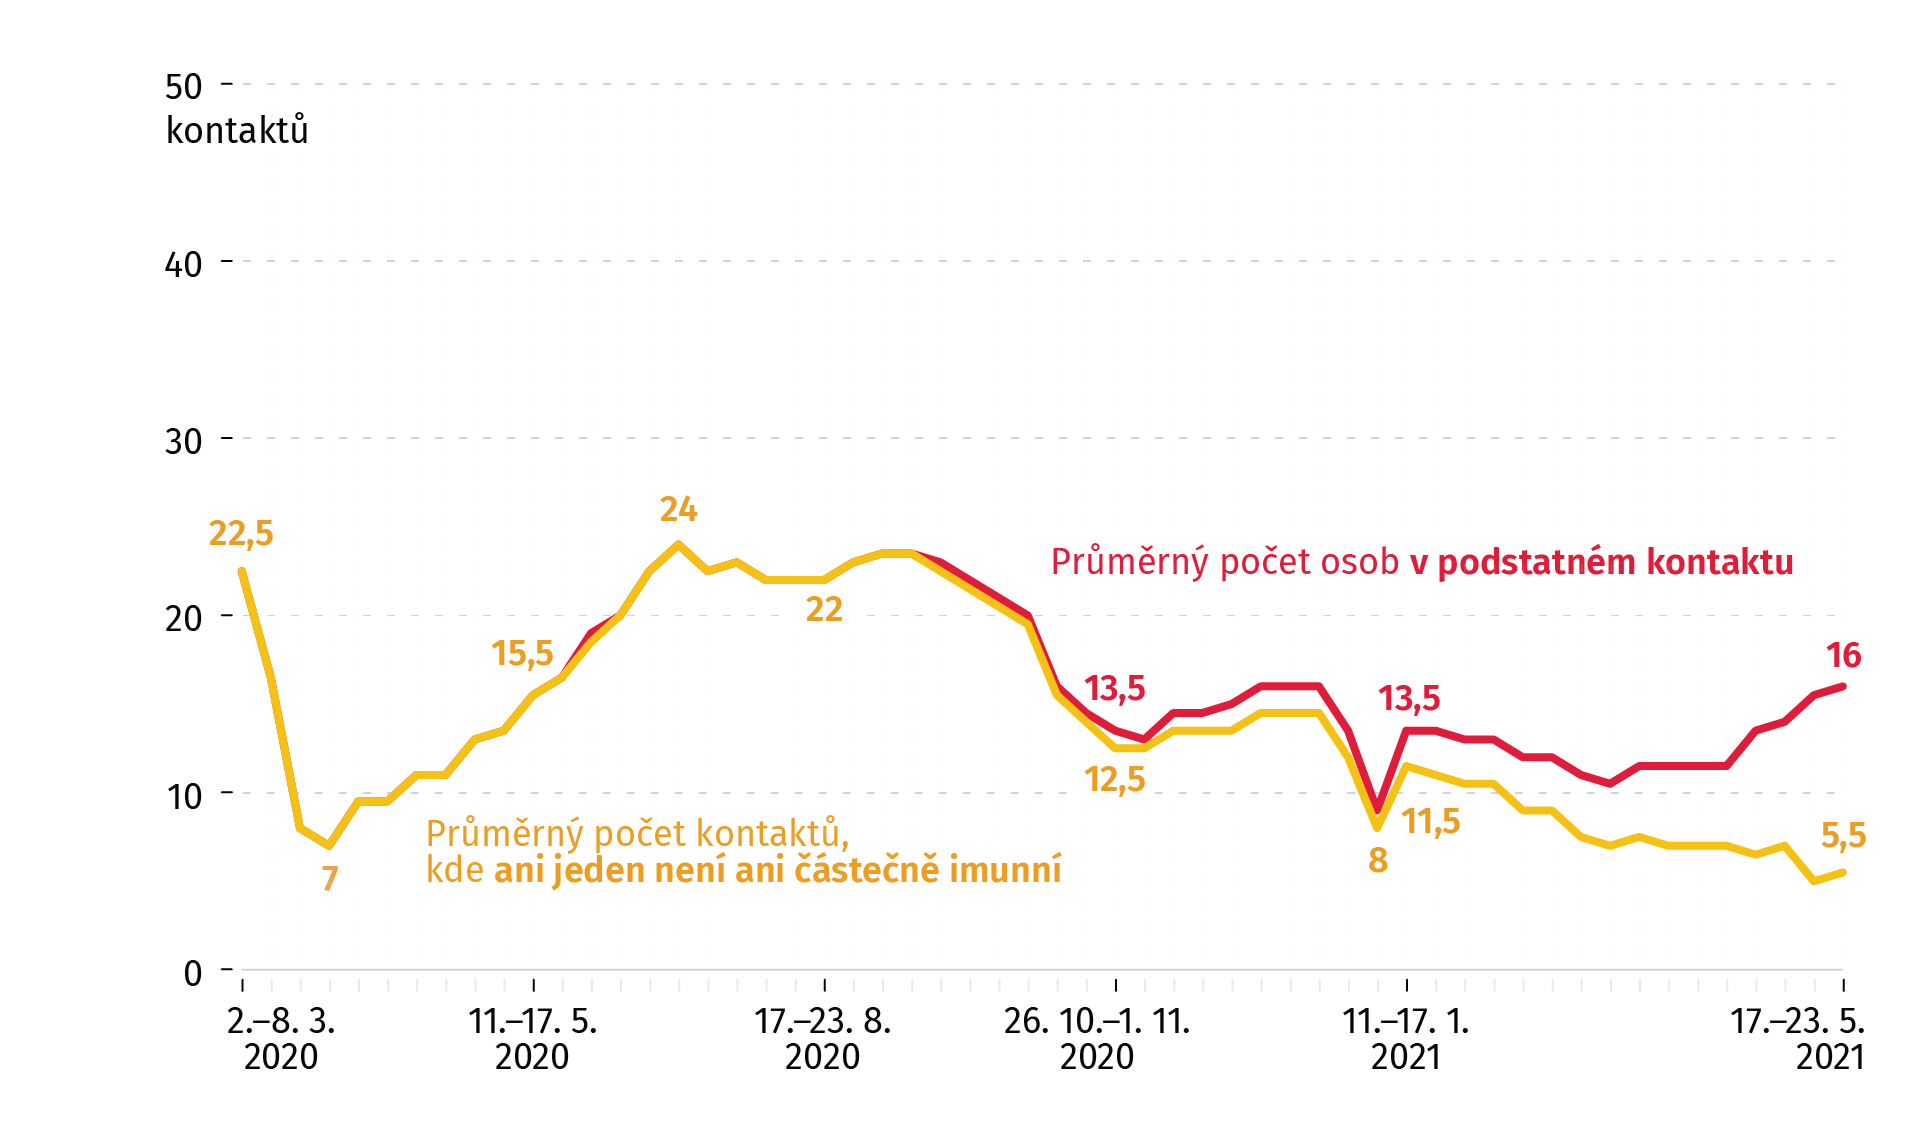
\includegraphics[width=\textwidth]{./pic/zbp-graf7.png}
    \caption{Vývoj odhadovaného počtu kontaktů (osobně, min. 5 minut) – v daných týdnech.}
    \label{fig:zbp7}
\end{figure}

Více informací a výsledky pro skupiny obyvatel viz: \url{https://zivotbehempandemie.cz/kontakty}

Vývoj očkování a s ním i imunizace společnosti přispěly k~\uv{brždění} epidemie na jaře 2021. Rizika však lze vidět v tom, že velká část zbývající nenaočkované populace má různé typy bariér (lidé nad 55 let) či omezenou ochotu (do 54 let bez maturity). Velká část populace tou dobou měla pouze první dávku očkování, k níž často měla i pragmatické důvody, a nelze vyloučit nárůst počtu lidí nedocházejících na druhou dávku. Míra aktivit a kontaktů už také koncem května směřovala ke stavu plně mimo epidemii, kterého zřejmě dosáhne až v průběhu června.

\section*{Závěrem}

Analýza dat \uv{Života během pandemie} ukazuje, že epidemie covid-19 v Česku měla dopady, které sahají za to, co známe z běžných statistik. Kromě nárůstu ne\-za\-měst\-na\-nos\-ti, který byl omezený, se v některých obdobích až 20\,\% lidí potýkalo s kompenzovaným či nekompenzovaným omezením práce. Zatímco řadu skupin společnosti epidemie ekonomicky nezasáhla, nebo se jejich příjmy a úspory i zvýšily, výrazně negativní dopady měla na lidi pracující v nestabilních úvazcích (dohody, příjmy tzv. na ruku) – nejčastěji v oblasti služeb. Výrazné dopady na duševní zdraví ukazuje nárůst symptomů depresí a úzkostí zejména u~žen s dětmi v domácnosti, mladých lidí a ekonomicky zasažených lidí.

I~pro pochopení vývoje epidemie jsou potřeba sociologické výzkumy. V Česku ukazují například relativně omezené využívání home office a velmi krátkodobou redukci setkávání se s širší rodinou a přáteli, která ve většině vln epidemie trvala jen zhruba 1,5 měsíce. Modelování ze sociologických dat přitom ukazuje, že právě při setkávání s přáteli a rodinou a v práci se odehrávala většina kontaktů – a to zejména v době, kdy řada volnočasových aktivit byla omezena. Toto modelování může také dávat návod, kde existuje místo pro efektivní protiepidemická opatření. Již od konce podzimu například bylo zřejmé, že musí cílit na omezení rizikovosti přenosu v zaměstnání, kde se v době restrikcí volného času a sociálního života odehrávala téměř polovina sociálních kontaktů.

Sociologická data jsou ale klíčová i pro plánování očkování a kampaní na jeho podporu – už v průběhu jara ukazovala dva potenciální problémy. Prvním jsou bariéry části starší a méně vzdělané populace v přístupu k očkování, kdy roli může hrát nižší digitální gramotnost a informovanost, podpora okolí (méně vzdělaní senioři mají často méně vzdělané děti, které očkování častěji nevěří), menší důvěra k expertům/institucím, schopnost dojíždět i menší očekáváné výnosy. Druhým je omezená ochota lidí do 54 let bez maturity k očkování. Řešení těchto dvou problémů přitom vyžaduje zcela odlišné přístupy.

Výrazně vyšší míra nadměrných úmrtí v postkomunistické Evropě má vedle zdravotních příčin pravděpodobně také sociální.\footnote{Podrobně se jim věnuje esej Daniela Prokopa v~Salonu Práva: \url{https://www.novinky.cz/kultura/salon/clanek/esej-daniela-prokopa-proc-vychod-prohrava-s-covidem-40354453}} Patří mezi ně průmyslová struktura ekonomiky a omezené možnosti využívání home office, výrazné zastoupení vícegeneračních domácností (průměrný věk odchodu z domova je v postkomunistické Evropě mezi 26 a 31 lety a ve Skandinávii mezi 18 a 21 lety), a tím snazší mezigenerační přenos viru. Ale také restriktivnější nastavení veřejných politik (náhradový poměr v karanténách a izolacích s covid-19 okolo 60\,\% odrazující od testování) a související nižší důvěra k~institucím, s~výraznějším projevem při dlouho trvající epidemii.

Úkolem sociologických pracovišť do dalších let by mělo být popsat tyto slabé stránky české společnosti, které zvyšují zranitelnost při epidemiích, a pokračovat v tvorbě longitudinálních studií jako \uv{Život během pandemie}, které mimo popsané výstupy umožňují i modelování vlivu jednotlivých aktivit na pravděpodobnost na\-ka\-že\-ní či popisují vztah dopadů pandemie na ekonomiku a duševní zdraví a poklesu ochoty dodržovat protiepidemická opatření.